\documentclass{standalone}
\usepackage{tikz}
\begin{document}
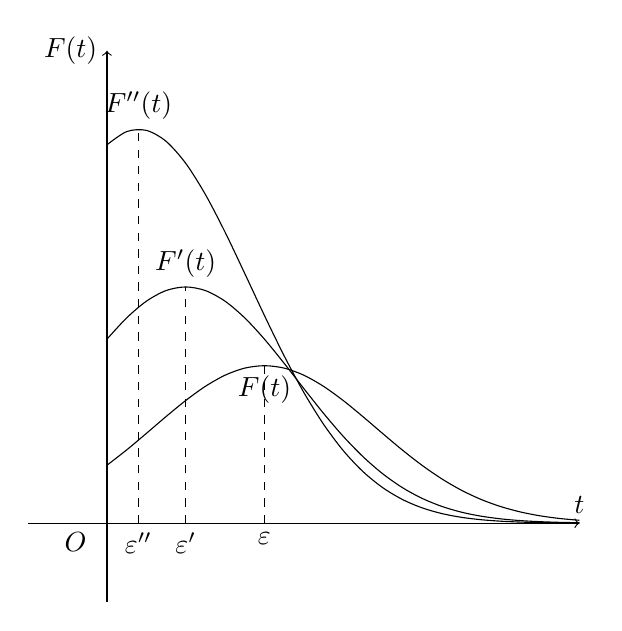
\begin{tikzpicture}[scale=2]
    \draw[->](-0.5,0)--(3,0)node[above]{$t$};
    \draw[->](0,-0.5)--(0,3)node[left]{$F(t)$};
    \node[below]at(-0.2,0){$O$};

    \draw[-]plot[smooth,domain=0:3](\x,{e^-((\x-1)^2)});
    \draw[-]plot[smooth,domain=0:3](\x,{1.5*e^-((\x-0.5)^2)});
    \draw[-]plot[smooth,domain=0:3](\x,{2.5*e^-((\x-0.2)^2)});
    
    \node[above]at(0.2,2.5){$F''(t)$};
    \draw[dashed](0.2,0)node[below]{$\varepsilon''$}--(0.2,2.5);
    \node[above]at(0.5,1.5){$F'(t)$};
    \draw[dashed](0.5,0)node[below]{$\varepsilon'$}--(0.5,1.5);
    \node[below]at(1,1){$F(t)$};
    \draw[dashed](1,0)node[below]{$\varepsilon$}--(1,1);
\end{tikzpicture}
\end{document}